\documentclass{scndocument}
\usepackage[utf8]{inputenc}
\usepackage{multicol}
\usepackage{import}
\usepackage{graphicx}
\usepackage{scn}
\linespread{0.9}
\usepackage[left=2.5cm, right=3cm, top=2.1cm, bottom=2.5cm]{geometry}
\graphicspath{ {./images/} }

\begin{document}
\begin{multicols}{2}
\noindent glossary. Hence, it is important to consider the structure to be formed by this agent, i.e. the principles and rules by which this agent should form the structure of the \textit{OSTIS Glossary}.

In this section, the authors of this paper also want to focus only on why it is important and how to structure and stratify information in general. That is, the purpose of this section is to review the principles of structuring
and stratification of knowledge in knowledge bases on \textit{SC-code},  because as it was clarified earlier, the \textit{OSTIS Glossary} is part of one common knowledge base of one ostis-system. If necessary, a detailed description of the syntax and denotational semantics of the knowledge
representation language can be found in the works of [34], [41], and a detailed description of what knowledge is and how to structure knowledge in knowledge bases can be found in the works of the following authors [42].

So, let us consider in detail the listed structuring principles of the \textit{OSTIS Standard} and describe the structuring principles of the \textit{OSTIS Glossary}.

In the context of the \textit{OSTIS Standard} usually defined as either a concept, i.e. an abstract entity that combines other abstract or concrete entities, or an instance of a concept, i.e. a concrete entity. Concepts
can be absolute or relative. Absolute concepts denote the same attributes of some group of concepts or entities, relative concepts — connections and relations between other concepts or entities. Generally speaking, there are
quite a lot of types of knowledge that can be represented on the \textit{SC-code}.  Absolute and relative concepts are basic characteristics of other concepts.

The specification of an object is commonly used to denote a set of information describing this object. Depending on the quality of the knowledge base, primarily determined by the quality of its development, concepts and entities can be specified or unspecified.

Suitably specified entities have the following requirements: 

\begin{itemize}
    \item if the entity is not a concept, the following must be
specified for it:
    \begin{itemize}
        \item different variants of the external signs denoting it;
    \end{itemize}
    \begin{itemize}
        \item the classes to which it belongs;
    \end{itemize}
    \begin{itemize}
        \item the links by which it is connected to other entities (indicating the relevant relationship);
    \end{itemize}
    \begin{itemize}
        \item values of the parameters it possesses;
    \end{itemize}
    \begin{itemize}
        \item those sections of the knowledge base in which the specified entity is key;
    \end{itemize}
    \begin{itemize}
        \item the subject domains in which the entity is included;
    \end{itemize}
    
\end{itemize}

\begin{itemize}
    \item if the specified entity is a concept, the following must be specified for it:
    \begin{itemize}
        \item different variants of external labelling of this concept;
    \end{itemize}
    \begin{itemize}
        \item The subject domains in which this concept is explored;
    \end{itemize}
    \begin{itemize}
        \item definition of the concept;
    \end{itemize}
    \begin{itemize}
        \item explanation;
    \end{itemize}
    \begin{itemize}
        \item sections of the knowledge base in which this concept is key;
    \end{itemize}
    \begin{itemize}
        \item example description - an example of an instance of a concept.
    \end{itemize}
\end{itemize}
These requirements can be formulated in another way. For each object in the knowledge base it is possible to fix their specifications by means of structures denoting sets of all relations of these objects with other objects
in the knowledge base. For these structures it is possible to introduce classification, i.e. to set classes for these structures, with the help of which it is possible to understand the degree of detail of specification of a
particular object of the knowledge base.

Within the framework of the \textit{OSTIS Technology}  for each entity it is done so, such structures describing the specification of entities in the knowledge base are commonly called semantic neighbourhood. Semantic neighbourhood is a specification of a given entity, the sign of which is specified as a key element of this specification.

The set of features by which entities can be specified varies. In addition, it may be necessary to specify the same entity in different aspects and to explicitly capture athese aspects in the knowledge base (Fig. 1).

For example, the same person can be described from professional, medical, civil and other perspectives, as presented in the figure.

Consider a specific example of the concept of "cybernetic system" and its specification from the \textit{OSTIS Standard}.
\newline
\newline 

\begin{scn}
    \scnheader{cybernetic system}
    \scnidtf{adaptive system}
    \scnidtf{targeted system}
    \scnidtf{active subject of independent activity}
    \scnidtf{a material entity capable of purposefully (in its
own interests) influencing its environment as a
minimum to preserve its integrity, viability, and
safety}
    \scnidtf{a natural or artificially created system capable of
monitoring and analysing its own state and the
state of the environment, as well as capable of
sufficiently active influence on its own state and
the state of the environment}
\scnidtf{information processing based system}
\begin{scnrelfromset}{note}
The level of adaptability, purposefulness, activity
in systems based on information processing can
be very different.

\end{scnrelfromset}
    
\end{scn}




\par
\end{multicols}
\newpage

\begin{multicols}{2}
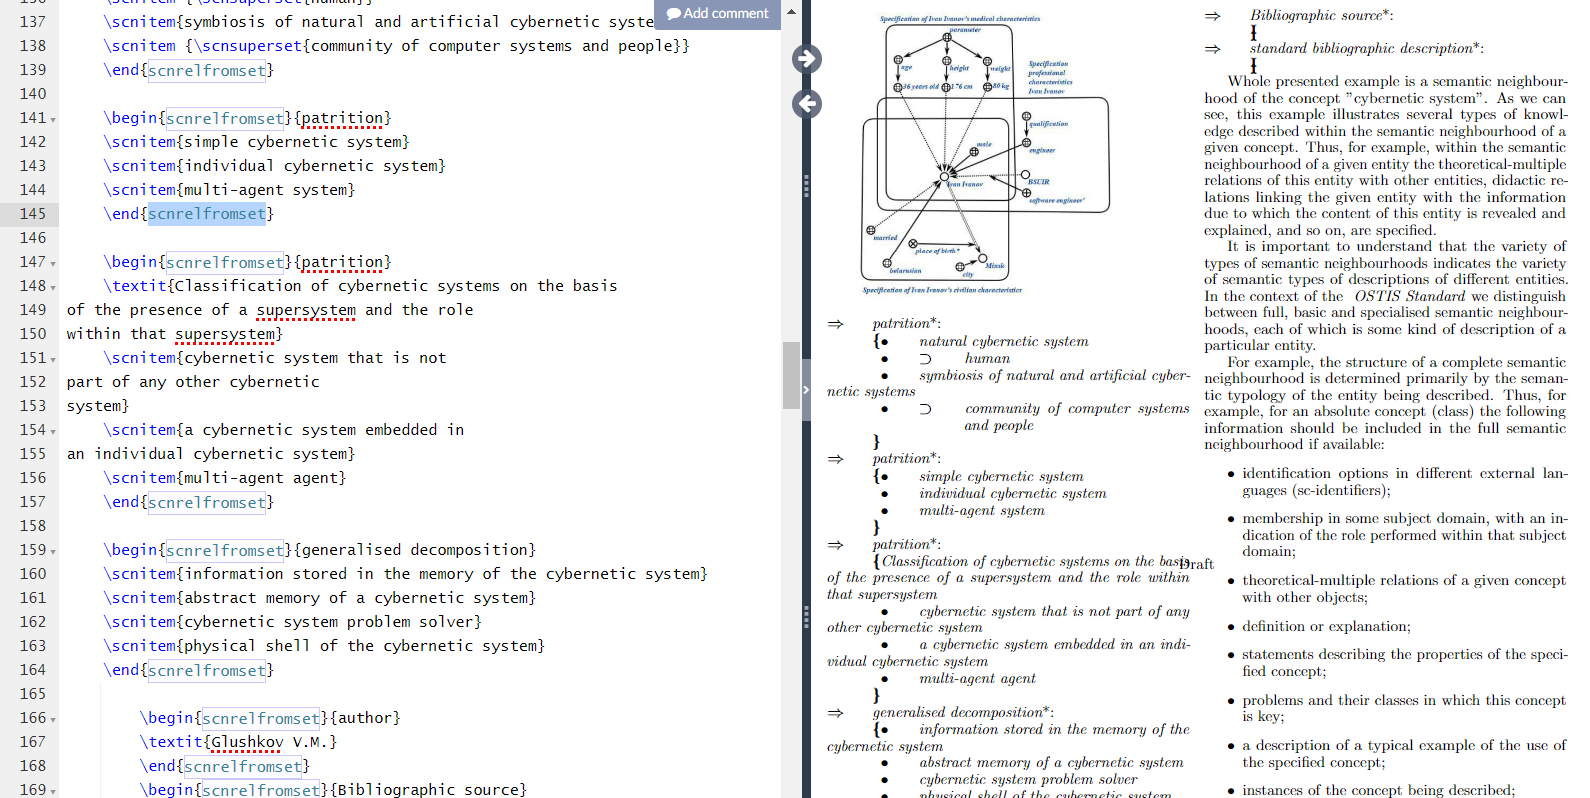
\includegraphics[scale = 0.5]{image.png}
\begin{figure}
    \centering
    \includegraphics[width=0.5\linewidth]{}
    \caption{Caption}
    \label{fig:enter-la bel}
\end{figure}
\par

\newline
\newline

\normalsize
\begin{scn}
    \begin{scnrelfromset}{patrition}
    \scnitem{natural cybernetic system}
    \scnitem {\scnsuperset{human}}
    \scnitem{symbiosis of natural and artificial cybernetic systems}
    \scnitem {\scnsuperset{community of computer systems and people}}
    \end{scnrelfromset}

    \begin{scnrelfromset}{patrition}
    \scnitem{simple cybernetic system}
    \scnitem{individual cybernetic system}
    \scnitem{multi-agent system}
    \end{scnrelfromset}

    \begin{scnrelfromset}{patrition}
    \textit{Classification of cybernetic systems on the basis
of the presence of a supersystem and the role
within that supersystem}
    \scnitem{cybernetic system that is not
part of any other cybernetic
system} 
    \scnitem{a cybernetic system embedded in
an individual cybernetic system}
    \scnitem{multi-agent agent}
    \end{scnrelfromset}

    \begin{scnrelfromset}{generalised decomposition}
    \scnitem{information stored in the memory of the cybernetic system}
    \scnitem{abstract memory of a cybernetic system}
    \scnitem{cybernetic system problem solver}
    \scnitem{physical shell of the cybernetic system}
    \end{scnrelfromset}

        \begin{scnrelfromset}{author}
        \textit{Glushkov V.M.}
        \end{scnrelfromset}
        \begin{scnrelfromset}{Bibliographic source}
        \end{scnrelfromset}
        \begin{scnrelfromset}{standard bibliographic description}
        \end{scnrelfromset}
    
    
\end{scn}

 
 

\newline


Whole presented example is a semantic neighbourhood of the concept "cybernetic system". As we can see, this example illustrates several types of knowledge described within the semantic neighbourhood of a given concept.
Thus, for example, within the semantic neighbourhood of a given entity the theoretical-multiple relations of this entity with other entities, didactic relations linking the given entity with the information due to which the
content of this entity is revealed and explained, and so on, are specified.

It is important to understand that the variety of types of semantic  neighbourhoods indicates the variety of semantic types of descriptions of different entities. In the context of the \textit{ OSTIS Standard} we distinguish between full, basic and specialised semantic neighbourhoods, each
of which is some kind of description of a particular entity.

For example, the structure of a complete semantic neighbourhood is determined primarily by the semantic typology of the entity being described. Thus, for example, for an absolute concept (class) the following information should be included in the full semantic neighbourhood if available:
\begin{itemize}
    \item  identification options in different external languages (sc-identifiers);
    \item membership in some subject domain, with an indication of the role performed within that subject domain;
    \item theoretical-multiple relations of a given concept with other objects;
    \item definition or explanation;
    \item statements describing the properties of the specified concept;
    \item problems and their classes in which this concept is key;
    \item a description of a typical example of the use of the specified concept;
    \item  instances of the concept being described;
    \item authors and bibliographic sources of the specified concept;
    \item and others.


\end{itemize}

\end{multicols}

\newpage

\begin{multicols}{2}
    For a relative concept, i.e. a concept that is a relation, the semantic neighbourhood additionally specifies:
\begin{itemize}
    \item domains;
    \item area of definition;
    \item relationship diagram;
    \item classes of relations to which the described relation belongs.
\end{itemize}

Obviously, there can be a large number of types of such specifications, since there can be a lot of information describing a particular object, and the need to obtain and visualise this information can be different. For the \textit{OSTIS Glossary}, too, it is possible to specify a kind of semantic neighbourhood, with the help of which it will be possible to specify only what is important from the point of view of the \textit{OSTIS Glossary} itself.

Drawing an analogy with the \textit{OSTIS Standard}, all inrformation in the \textit{OSTIS Glossary} can be presented in the form of ordered and organized sections of the subject domains and ontologies that make up the \textit{OSTIS
Standard.} Each section can be presented as a sequence of objects and their specifications arranged alphabetically by the terms of these objects, i.e. in lexicographic order.

In the context of the \textit{OSTIS Glossary}, the specification of each object \underline{should} specify:
\begin{itemize}
    \item identification options in various external languages (sc-identifiers);
    \item object membership in some subject domain with indication of the role performed within this subject domain;
    \item theoretical-multiple relations of a given object with other objects;
    \item definition or explanation of a given object;
    \item description of a typical example of the use of the specified object;
    \item instances of the described object, if the given object is a concept;
    \item authors of the given object;
    \item authors of the specification of the given object;
    \item analogs of the given object;
    \item bibliographic sources of the object.
    \end{itemize}

    In other words, in the context of the \textit{OSTIS Glossary}, the semantic neighborhood of each specifiable object should include not just information defining and explaining the specified object, but also the information that determines the level of significance of this object in comparison with other objects. In this case, the \textit{OSTIS Glossary} acts not only as a tool for consistency of some kind of activity, but also plays an important role in search and comparison of similar objects, i.e. it acts as a tool for convergence of different, but having common features, objects.
    
    Thus, with the help of semantic neighborhoods it is possible to structure ("horizontally") knowledge about other knowledge. In order to stratify ("vertically") this knowledge about other knowledge among themselves, other kinds of structures have to be used. Therefore, all the \textit{OSTIS Standard} objects are grouped by subject domains and their corresponding ontologies, which are used to stratify knowledge in knowledge bases.

    The concept of the subject domain is the most important methodological technique, which allows to single out from the whole variety of the investigated World only a certain class of investigated entities and only a certain family of relations defined on the specified class. That is, localization, focusing attention only on it, abstracting from the rest of the World under study, is carried out.

    The subject domains and their corresponding ontologies identified within the knowledge base of an intelligent system are semantic strata, clusters, which allow to "decompose" all the knowledge stored in the memory into "semantic shelves" in the presence of clear criteria that allow to unambiguously determine on which "shelf" certain knowledge should be located.

    From the point of view of the \textit{OSTIS Standard}, a subject domain is the result of integration (union) of partial semantic neighborhoods describing all investigated entities of a given class and having the same (common) subject of investigation (i.e. the same set of relations to which the mappings belonging to the integrated semantic neighborhoods should belong). That is, the subject domain is a structure that includes:
    \begin{itemize}
        \item the main studied (described) objects — primary and secondary;
        \item different classes of studied objects;
        \item different links, the components of which are the studied objects;
        \item different classes of the above-mentioned links (i.e. relations);
        \item different classes of objects that are neither the studied objects nor the above-mentioned links, but are components of these links.
    \end{itemize}

    Each concept corresponds to at least one subject domain in which the concept is a studied concept and in which the main characteristics of the concept are dealt with. When describing any subject domain, it is important that all classes declared by the studied concepts should be fully represented within the given subject domain together with their elements, elements of elements, etc. up to terminal elements.

    For effective collective development and operation of the knowledge base of the ostis-system not just structuring is important, but such structuring, which is as objective as possible, having a clear semantic interpretation and allowing, on the basis of semantic links between
structurally selected fragments of the knowledge base, to easily determine (localise) the "location" of either the knowledge being sought or new knowledge being introduced into the knowledge base. Such semantic structuring of the knowledge base, the formation of a system of semantically related "semantic shelves" on which spe-
\end{multicols}

\newpage

\end{document}